\chapter{Graph Colourings}

% Disclaimer (Unnumbered Header)
\par\vspace{0.5cm}\noindent
\needspace{3\baselineskip}
{\large \underline{\textbf{Disclaimer}}}
\par\vspace{0.2cm}
The title is actually somewhat misleading, as our first convention will be that we can understand different colours simply as different positive integers. Hence we will use the ``colours'' $1, 2, 3, \dots$ instead of red, blue, brown etc. Visualisations can nevertheless reassociate these numbers with colours.

\section{The Chromatic Number}

% 6.1 Definition
\begin{definition}
Let $G$ be a graph. A \textbf{\color{red}$k$-colouring} is a function $K: V_G \to \{1, 2, \dots, k\}$ for $k \in \mathbb{Z}_+$ s.t. $K(x) = K(y)$ implies $xy \notin E_G$, i.e. adjacent vertices receive distinct colours. We call $\{1, 2, \dots, k\}$ the \textbf{\color{red}colours} of $K$. We say that $K$ is a \textbf{\color{red}colouring} of $G$ if it is a $k$-colouring for some $k$ and we call $G$ \textbf{\color{red}$k$-colourable} if there is a $k$-colouring for $G$.
\end{definition}

% 6.2 Remarks
\begin{remark}
Let $G$ be any graph.
\begin{enumerate}
    \item[1)] If $G$ is $k$-colourable, then it is $j$-colourable for any $j \ge k$.
    \item[2)] If $K$ is a $k$-colouring of $G$, then $V_r := K^{-1}(r) = \{v \in V_G \mid K(v)=r\}$ is an independent subset of $G$ for any $r \in \{1, 2, \dots, k\}$.
    \item[3)] Every graph of order $n$ is clearly $n$-colourable as for $V_G = \{v_1, v_2, \dots, v_n\}$ we can simply define the injective function $K: V_G \to \{1, 2, \dots, n\}$ via $K(v_i)=i$. Any injective such function is clearly a colouring.
    \item[4)] Remarks 2) and 3) indicate that the interesting question will be to find small $k$ s.t. $G$ is $k$-colourable.
\end{enumerate}
\end{remark}

% 6.3 Example
\begin{example}
Consider the graph $C_5$. Let's try to find a minimal $k$ s.t. $G$ is $k$-colourable.
\begin{center}
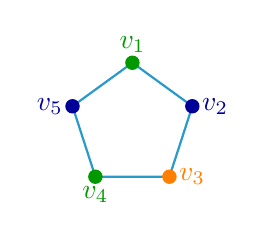
\begin{tikzpicture}[scale=0.8]
    \foreach \i in {1,...,5} \coordinate (v\i) at (90+72-72*\i : 1);
    \draw[cyan!80!black, thick] (v1)--(v2)--(v3)--(v4)--(v5)--(v1);
    
    % Colors based on note intuition (Green/Blue/Pink/Orange)
    \filldraw[green!60!black] (v1) circle (3pt) node[above] {$v_1$};
    \filldraw[blue!60!black] (v2) circle (3pt) node[right] {$v_2$};
    \filldraw[orange] (v3) circle (3pt) node[right] {$v_3$};
    \filldraw[green!60!black] (v4) circle (3pt) node[below] {$v_4$};
    \filldraw[blue!60!black] (v5) circle (3pt) node[left] {$v_5$};
\end{tikzpicture}
\end{center}
$\Rightarrow$ It seems we need at least 3-colours. $C_5$ is 3-colourable, as $K: V_G \to \{1, 2, 3\}$ via $K(v_1)=K(v_4)=1$, $K(v_2)=K(v_5)=2$ and $K(v_3)=3$ is a 3-colouring for $G$. We also could have defined $K$ via $V_1=\{v_1, v_4\}$, $V_2=\{v_2, v_5\}$ and $V_3=\{v_3\}$.
\end{example}

% 6.4 Remarks
\begin{remark}
\begin{enumerate}
    \item[1)] Note that every $k$-colouring $K$ of $G$ gives rise to a partition of $V_G$ into sets $V_1, V_2, \dots, V_k$ s.t. no two vertices in $V_i$ are adjacent. $G$ is hence $k$-partite. Note that $V_i$ could be empty for some $i$.
    \item[2)] As each $V_i$ is an independent set, we get $k \ge \frac{|G|}{\alpha(G)}$ (HW).
\end{enumerate}
\end{remark}

% 6.5 Definition
\begin{definition}
The \textbf{\color{red}chromatic number $\chi(G)$} of a graph $G$ is the smallest positive integer $k \in \mathbb{Z}_+$ s.t. $G$ is $k$-colourable.
\end{definition}

% 6.6 Examples
\begin{example}
\begin{enumerate}
    \item[1)] $\chi(G)=1$ iff $G=E_n$ is the empty graph for some $n$.
    \item[2)] $\chi(K_n)=n$, as all of the $n$-many vertices are pairwise adjacent.
    \item[3)] $\chi(K_{n,m})=2$, as we can colour each part of the partition in one colour.
    \item[4)] $\chi(P_n)=2$ for $n \ge 2$.
    \item[5)] $\chi(C_n) = \begin{cases} 2 & \text{if } n \text{ is even} \\ 3 & \text{otherwise} \end{cases}$ (HW).
\end{enumerate}
\end{example}

% 6.7 Remark
\begin{remark}
\begin{enumerate}
    \item[1)] $G$ is $k$-colourable iff $k \ge \chi(G)$.
    \item[2)] $\frac{|G|}{\alpha(G)} \le \chi(G) \le |G|$ for any graph $G$.
    \item[3)] $G$ is 2-colourable iff $G$ is bipartite (iff $\chi(G) \le 2$).
    \item[4)] If $F$ is a forest, then $\chi(F)=2$.
    \item[5)] If $H \subseteq G$ is a subgraph of $G$, then $\chi(H) \le \chi(G)$.
\end{enumerate}
\end{remark}

% 6.8 Definition
\begin{definition}
Let $n_1, \dots, n_k \in \mathbb{Z}_+$ be positive integers, $k \ge 1$. The \textbf{\color{red}complete $k$-partite graph $K_{n_1, n_2, \dots, n_k}$} is the graph whose vertex set is the disjoint union of $k$-many pairwise disjoint sets $V_1, \dots, V_k$ with $|V_i|=n_i$; and edge set $E = \{uv \mid u \in V_i, v \in V_j, i \ne j\}$. If we don't care about the specific value of $k$, we call $K_{n_1 \dots n_k}$ the \textbf{\color{red}complete multipartite graph}.
\end{definition}

% 6.9 Example
\begin{example}
The complete 3-partite graph $K_{3,1,2}$ is
\begin{center}
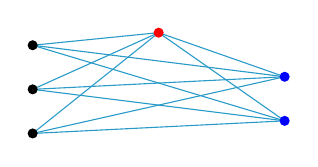
\begin{tikzpicture}[scale=0.8]
    % V1: 3 nodes (left)
    \foreach \i in {1,2,3} \coordinate (l\i) at (0, 2 - 0.7*\i);
    % V2: 1 node (center)
    \coordinate (c) at (2, 1.5);
    % V3: 2 nodes (right)
    \foreach \i in {1,2} \coordinate (r\i) at (4, 1.5 - 0.7*\i);
    
    % Edges: l to c, l to r, c to r
    \foreach \i in {1,2,3} {
        \draw[cyan!80!black] (l\i)--(c);
        \foreach \j in {1,2} \draw[cyan!80!black] (l\i)--(r\j);
    }
    \foreach \j in {1,2} \draw[cyan!80!black] (c)--(r\j);
    
    \foreach \p in {l1,l2,l3} \filldraw (\p) circle (2pt);
    \filldraw[red] (c) circle (2pt);
    \foreach \p in {r1,r2} \filldraw[blue] (\p) circle (2pt);
\end{tikzpicture}
\end{center}
We see that even for small numbers, the graph is difficult to draw. For which $n_1 \dots n_k$ is $K_{n_1 \dots n_k}$ planar?
\end{example}

% 6.10 Lemma
\begin{lemma}
Let $G$ be a graph and $k \ge 1$. Then $G$ is $k$-colourable iff $G$ is a subgraph of a complete $k$-partite graph.
\end{lemma}

\begin{proof}
$G$ is $k$-colourable \\
iff ex. $K: V_G \to \{1, 2, \dots, k\}$ s.t. $K(u)=K(v) \implies uv \notin E_G$ \\
iff ex. $K: V_G \to \{1, 2, \dots, k\}$ s.t. $K^{-1}(i)$ is an independent set (or empty) for all $i$ \\
iff we can partition $V_G$ into $k$-many independent sets $V_1, \dots, V_k$ ($V_i = \emptyset$ allowed) \\
iff $G$ is a subgraph of $K_{n_1 \dots n_k}$ for some $n_1 \dots n_k \in \mathbb{Z}_+$. \qedhere
\end{proof}

Next we want to introduce a greedy algorithm for finding a vertex colouring of a given graph. This algorithm is more efficient than giving every vertex a different colour, but it does not always produce a $\chi(G)$-colouring.

% 6.11 The Greedy Algorithm
\topic{The Greedy Algorithm}
Let $G$ be a graph of order $n$.
\begin{enumerate}
    \item[1)] Label the vertices by $v_1, \dots, v_n$.
    \item[2)] Fix the set of available colours to be $\{1, 2, \dots, n\}$.
    \item[3)] Let $i=1$.
    \item[4)] While $i \le n$
    \begin{itemize}
        \item Colour $v_i$ with the smallest available colour not used on any of its previously coloured neighbours, i.e. set
        \[ K(v_i) = \min \{ \{1, \dots, n\} \setminus \{K(v_j) \mid j < i, v_j \in N(v_i)\} \}. \]
        \item Set $i \to i+1$.
    \end{itemize}
\end{enumerate}

% 6.12 Lemma
\begin{lemma}
Let $G$ be a graph and $K$ be a colouring function produced by the greedy algorithm applied to $G$. Then for all $v \in V_G$, we get
\[ K(v) \le \deg(v) + 1. \]
\end{lemma}

\begin{proof}
We do induction on $|G|=n$. For $n=1$, clearly $G=K_1$, and $K(v_1) = 1 = \deg(v_1)+1$. Now assume the claim holds for any graph of order at most $n$ and consider $G$ with $|G|=n+1$.
Run the greedy algorithm on $G$. After the first $n$ rounds, we obtain a ``greedy'' colouring of $G-v_{n+1}$, whence $K(v_i) \le \deg^{G-v_{n+1}}(v_i) + 1 \le \deg^G(v_i) + 1$ for all $1 \le i \le n$. Now we run the last round and assign $K(v_{n+1}) = \min \{ \{1, \dots, n\} \setminus \{K(v_j) \mid v_j \in N(v_{n+1})\} \}$.
At most $\deg(v_{n+1})$-many colours have been used on its neighbours, whence among $\{1, 2, \dots, \deg(v_{n+1}), \deg(v_{n+1})+1\}$, there is at least one colour available. As the algorithm picks the smallest available colour, we conclude $K(v_{n+1}) \le \deg(v_{n+1}) + 1$, as desired.
\end{proof}

% 6.13 Corollary
\begin{corollary}
For any graph $G$ we have $\chi(G) \le \Delta(G) + 1$.
\end{corollary}

\begin{proof}
Apply the greedy algorithm on $G$. Then for any $v \in V_G$, we get $K(v) \le \deg(v) + 1 \le \Delta(G) + 1$, whence $K: V_G \to \{1, 2, \dots, \Delta(G)+1\}$ and $\chi(G) \le \Delta(G) + 1$.
\end{proof}

Finding the chromatic number of a graph is a very important, but computationally hard problem. It is known to be NP-hard and its best runtime is in $\mathcal{O}(2^n)$. We hence need to establish good bounds to approach the problem effectively.

% 6.14 Remark
\begin{remark}
\begin{itemize}
    \item For any graph $G$ we have $\chi(G) \le \Delta(G) + 1$.
    \item The bound is sharp, as
    \begin{itemize}
        \item $\chi(K_n) = n = (n-1)+1 = \Delta(K_n)+1$ for all $n \in \mathbb{Z}_+$ and
        \item $\chi(C_n) = 3 = 2+1 = \Delta(C_n)+1$ for all odd $n \in \mathbb{Z}_+$.
    \end{itemize}
    \item But are there more examples to witness that the bound is sharp (i.e. cannot be improved)? \textbf{\color{red}No.}
    \item Note: What do $C_n$ and $K_n$ have in common? They are regular!
\end{itemize}
\end{remark}

Goal of this lecture:

% 6.15 Theorem (Brooks' Theorem)
\begin{theorem}[Brooks' Theorem, 1941]
If $G$ is a connected graph which is neither complete, nor an odd cycle, then $\chi(G) \le \Delta(G)$.
\end{theorem}

We will split the proof into several Lemmata. Set $\Delta(G) =: \Delta$.

% 6.16 Step 1 - Remark on Delta <= 2
\begin{lemma}[Step 1 - Remark on $\Delta \le 2$]
Theorem 6.15 holds for $\Delta \le 2$, as if $\Delta=0$, then $G=K_1$, and if $\Delta=1$, then $G=K_2$ is complete, which is excluded.
For $\Delta=2$, either $\delta(G)=\Delta=2$ and $G$ is an even cycle, whence $\chi(G)=2 \le \Delta(G)$ holds, or $\delta(G)=1$ and $G$ is a path of length at least 2, and again $\chi(G)=2 \le \Delta(G)$.
Thus, from now on, consider such $G$ which satisfy $\Delta(G) \ge 3$.
\end{lemma}
% 6.17 Step 2 - Lemma
\begin{lemma}[Step 2 - Lemma on non-regular graphs]
If $G$ from 6.15 is not regular, then $\chi(G) \le \Delta(G)$ (i.e. the theorem holds).
\end{lemma}
\begin{proof}
If $G$ is non-regular, then ex. $v \in V_G$ s.t. $\deg(v) < \Delta(G)$.
The idea is to introduce a smart colouring which uses at most $\Delta(G)$ many colours. Note that as $G$ is (finite and) connected, $ecc(v) = k < \infty$. Let $S_i := \{u \in V_G \mid d(u,v)=i\}$. Hence, $S_0=\{v\}$ and $S_k = \{u \in V_G \mid d(u,v) = ecc(v)\}$. Note further that for $1 \le i \le k$, every vertex $u \in S_i$ has at least one neighbour in $S_{i-1}$ (i.e. the predecessor of $u$ on a $vu$-path of shortest length).

\begin{center}
\begin{tikzpicture}[
    % Define styles for consistency
    setnode/.style={
        draw=gray!60, 
        line width=1.5pt, 
        ellipse, 
        minimum height=3.5cm, 
        minimum width=1.5cm
    },
    edge/.style={
        cyan!90!blue, 
        line width=1.2pt, 
        line cap=round
    },
    label/.style={
        font=\Large\sffamily, 
        text=black
    }
]

    % --- Nodes ---
    
    % The vertex v (S0)
    \coordinate (v) at (0,0);
    \fill[black] (v) circle (3pt) node[above left] {\Large $v$};
    \node[label] at (0, -3) {$S_0$};

    % Set S1
    \node[setnode] (s1) at (3.5, 0) {};
    \node[label] at (3.5, -3) {$S_1$};

    % Set S2
    \node[setnode] (s2) at (7, 0) {};
    \node[label] at (7, -3) {$S_2$};

    % Dots
    \node[label] at (10, 0) {$\dots$};
    \node[label] at (10, -3) {$\dots$};

    % Set Sk
    \node[setnode] (sk) at (13, 0) {};
    \node[label] at (13, -3) {$S_k$};

    % --- Edges ---

    % Edges from v to S1 (Fanning out)
    \draw[edge] (v) -- (s1.140);
    \draw[edge] (v) -- (s1.165);
    \draw[edge] (v) -- (s1.195);
    \draw[edge] (v) -- (s1.220);

    % Edges from S1 to S2 (Connecting sets)
    \draw[edge] (s1.15) -- (s2.165);
    \draw[edge] (s1.0) -- (s2.180);
    \draw[edge] (s1.345) -- (s2.195);

    % Edges from S2 outgoing (Partial lines)
    \draw[edge] (s2.15) -- ++(1.5, -0.0065);
    \draw[edge] (s2.0) -- ++(1.5, 0);
    \draw[edge] (s2.345) -- ++(1.5, 0.00195);

    % Edges entering Sk
    \draw[edge] ($(sk.165)+(-1.5, 0.2)$) -- (sk.165);
    \draw[edge] ($(sk.180)+(-1.5, 0)$) -- (sk.180);
    \draw[edge] ($(sk.195)+(-1.5, -0.2)$) -- (sk.195);

\end{tikzpicture}
\end{center}

We want to apply the greedy algorithm after labelling the vertices of $G$ in a smart way: We start by randomly labelling the vertices in $S_k$ and \underline{then} those in $S_{k-1}$ and so on and so forth until the last vertex $v$ gets labelled $v_n$ where $n=|G|$.
Hence, if $v_i \in S_\ell$ and $v_j \in S_m$ for $\ell < m$, then $i > j$.
Now we run the greedy algorithm and observe which colours the vertices get.
For $v_i \in S_\ell$ with $\ell \ne 0$ (i.e. $v_i \ne v_n = v$), note that $v_i$ gets the smallest available colour not used on its \underline{previously coloured} neighbours, i.e. on its neighbours in $S_\ell \cup S_{\ell+1} \cup \dots \cup S_k$.
As $v_i$ has at least one neighbour in $S_{\ell-1}$, these are at most $\deg(v_i)-1 \le \Delta(G)-1$ many. Hence, at least one of the colours $\{1, 2, \dots, \Delta(G)\}$ is still available, whence $K(v_i) \le \Delta(G)$ as desired.
For $v_n=v$, it gets the smallest available colour not used on \underline{any} of its neighbours, as it is the last to get coloured. But as by choice, $\deg(v_n) < \Delta(G)$, again one of the colours $\{1, 2, \dots, \Delta(G)\}$ must be available and $K(v_n) \le \Delta(G)$.
Hence, $K(u) \le \Delta$ for all $u \in V_G$, whence $G$ is $\Delta$-colourable and $\chi(G) \le \Delta$, as desired.
\end{proof}

% 6.18 Step 3
\begin{lemma}[Step 3 - Regular graphs with cut vertices]
Let $G$ be a connected, regular graph with $\Delta(G) \ge 3$. If $G$ contains a cut vertex (i.e. $\kappa(G)=1$), then $\chi(G) \le \Delta(G)$.
\end{lemma}
% 6.19 Example
\begin{example}
You might wonder if these graphs exist. Here is an example:
\begin{center}
\begin{tikzpicture}[
    % Style definitions
    vertex/.style={
        circle, 
        fill=black, 
        inner sep=1.5pt
    },
    edge/.style={
        cyan!80!blue, 
        line width=1.2pt, 
        line cap=round,
        line join=round
    },
    blob/.style={
        draw=gray!40, 
        line width=1.5pt, 
        tension=0.8
    },
    label/.style={
        text=gray!60, 
        font=\Large\sffamily
    }
]

    % --- Central Vertex ---
    \node[vertex] (v) at (0,0) {};
    \node[gray!60, below=0.2cm of v] {\large $v$};

    % ================= H1 (Left) =================
    % Coordinates
    \coordinate (L_conn) at (-1.5, 0.2); % Connector node
    \coordinate (L_topR) at (-3, 1.2);
    \coordinate (L_botR) at (-3, -0.8);
    \coordinate (L_topL) at (-5, 1.2);
    \coordinate (L_botL) at (-5, -0.8);

    % Vertices
    \node[vertex] (l1) at (L_conn) {};
    \node[vertex] (l2) at (L_topR) {};
    \node[vertex] (l3) at (L_botR) {};
    \node[vertex] (l4) at (L_topL) {};
    \node[vertex] (l5) at (L_botL) {};

    % Edges (Box with X)
    \draw[edge] (v) -- (l1);        % Stem to center
    \draw[edge] (l1) -- (l2);
    \draw[edge] (l1) -- (l3);
    \draw[edge] (l2) -- (l4) -- (l5) -- (l3) -- (l2); % Box
    \draw[edge] (l2) -- (l5);       % Cross 1
    \draw[edge] (l3) -- (l4);       % Cross 2

    % Blob H1
    \draw[blob] plot [smooth cycle] coordinates {
        (-0.2, -0.5) 
        (-1.5, -1.2) 
        (-5.5, -1.2) 
        (-5.5, 1.6) 
        (-1.5, 1.6) 
        (-0.2, 0.5)
    };
    \node[label] at (-5.5, 2) {$H_1$};


    % ================= H3 (Right) =================
    % Coordinates (Symmetric to H1)
    \coordinate (R_conn) at (1.5, 0.2);
    \coordinate (R_topL) at (3, 1.2);
    \coordinate (R_botL) at (3, -0.8);
    \coordinate (R_topR) at (5, 1.2);
    \coordinate (R_botR) at (5, -0.8);

    % Vertices
    \node[vertex] (r1) at (R_conn) {};
    \node[vertex] (r2) at (R_topL) {};
    \node[vertex] (r3) at (R_botL) {};
    \node[vertex] (r4) at (R_topR) {};
    \node[vertex] (r5) at (R_botR) {};

    % Edges
    \draw[edge] (v) -- (r1);
    \draw[edge] (r1) -- (r2);
    \draw[edge] (r1) -- (r3);
    \draw[edge] (r2) -- (r4) -- (r5) -- (r3) -- (r2);
    \draw[edge] (r2) -- (r5);
    \draw[edge] (r3) -- (r4);

    % Blob H3
    \draw[blob] plot [smooth cycle] coordinates {
        (0.2, -0.5) 
        (1.5, -1.2) 
        (5.5, -1.2) 
        (5.5, 1.6) 
        (1.5, 1.6) 
        (0.2, 0.5)
    };
    \node[label] at (5.5, 2) {$H_3$};


    % ================= H2 (Top) =================
    % Coordinates
    \coordinate (T_stem) at (0, 1.5);
    % Create a hexagon shape above
    \foreach \i in {1,...,6} {
        \coordinate (T\i) at ($(0, 3.2) + ({(\i-1)*60 + 90}:1.2)$);
    }

    % Vertices
    \node[vertex] (t_stem) at (T_stem) {};
    \foreach \i in {1,...,6} {
        \node[vertex] (vn\i) at (T\i) {};
    }

    % Edges
    \draw[edge] (v) -- (t_stem);
    \draw[edge] (t_stem) -- (vn4); % Connect stem to bottom of wheel

    % Wheel perimeter
    \draw[edge] (vn1) -- (vn2) -- (vn3) -- (vn4) -- (vn5) -- (vn6) -- (vn1);
    % Internal chords (Star)
    \draw[edge] (vn1) -- (vn4);
    \draw[edge] (vn2) -- (vn5);
    \draw[edge] (vn3) -- (vn6);

    % Blob H2
    \draw[blob] plot [smooth cycle] coordinates {
        (-0.6, 0.2)
        (-1.8, 2.5)
        (-1.5, 4.8)
        (1.5, 4.8)
        (1.8, 2.5)
        (0.6, 0.2)
    };
    \node[label] at (2, 4) {$H_2$};

    % Redraw v on top so lines don't cover it
    \node[vertex] at (0,0) {};

\end{tikzpicture}
\end{center}
All $H_i$ are non-regular.
\end{example}

\begin{proof}of 6.18:\\ Let $v$ be a cut vertex in $G$, i.e. $G-v$ is disconnected. Let $H_1, H_2, \dots, H_k$ be the distinct connected components of $G-v$ with $k \ge 2$. Further, define $G_i := \langle V(H_i) \cup \{v\} \rangle$ to be the graph induced on $H_i$ with $v$. Note that $\deg^{G_i}(v) < \deg^G(v) = \Delta$, while still $\deg(u) = \Delta$ for all other $u \in V(G_i)$. Hence $\Delta(G_i) = \Delta$. By Step 2, we can find $\Delta$-colouring of $G_i$. Possibly after permuting the colours, we may assume that $K_i(v) = K_j(v)$ for all $1 \le i,j \le k$.
Hence $K = K_1 \cup \dots \cup K_k$ is the desired $\Delta$-colouring of $G$. \qed
\end{proof}
% 6.20 Auxiliary Step 4 - Fact
\begin{lemma}[Step 4]
Suppose that $G$ is regular and $2$-connected with $\Delta(G) \geq 3$. Then there exist three vertices $v, v_1, v_2$ such that $v$ is adjacent to both $v_1, v_2$ where $v_1, v_2$ are nonadjacent, and $G - \{v_1, v_2\}$ is connected.
\end{lemma}

\begin{proof}
As $G$ is regular, every vertex has degree $\Delta$. To show this case we will divide this case into two subcases.

\paragraph{Case a.} Suppose that $G$ is regular and $3$-connected. \\
Since $G$ is regular and not complete, it follows that $\Delta < n - 1$. Let $v_1$ be any vertex of $G$ and let $A$ be the set of all vertices which are nonadjacent to $v_1$. As $\deg(v_1) = \Delta < n - 1$ there must be a vertex nonadjacent to $v_1$, and so $A \neq \emptyset$. Suppose for the moment that no neighbour of $v_1$ is adjacent to some vertex in $A$. But then there will be no path in $G$ from $v_1$ to any vertex in $A$ contradicting that $G$ is connected. Therefore, there exists some neighbour $v$ of $v_1$ which is adjacent to some vertex $v_2 \in A$. As $\kappa(G) \geq 3$, we know that $G - \{v_1, v_2\}$ is connected. This completes Case a.

\paragraph{Case b.} Suppose that $G$ is regular and $\kappa(G) = 2$. (This means $G$ is $2$-connected but not $3$-connected.) \\
This means that there are two vertices $v, w$ which form a cut set. So $G - \{v, w\}$ is disconnected. Let $G_1, G_2, \dots, G_t$ where $t \geq 2$ be the connected components of $G - \{v, w\}$. Since $\Delta \geq 3$, each $G_i$ must contain at least $2$ vertices. We will establish two facts.

\textbf{Claim 1.} The vertex $v$ has at least one neighbour in each $G_i$. \\
To see this, observe that $w$ is not a cut vertex of $G$ since $\kappa(G) = 2$. So $G - w$ is connected. Suppose that $v$ is not adjacent to any vertex in $G_i$ for some $i$. Let $x$ be a vertex in $G_i$, as $G - w$ is connected, there is $vx$-path $P$ in $G - w$. Since $v$ is nonadjacent to all vertices in $G_i$, the successor of $v$ in $P$ must be some vertex $z$ from $G_j$ where $j \neq i$. But then $P[z, x]$ is a path which does not use either $v$ or $w$. This shows that $G_i$ and $G_j$ are connected in $G - \{v, w\}$, a contradiction. Thus, the vertex $v$ must be adjacent to at least one vertex in each $G_i$ as required.

\textbf{Claim 2.} The vertex $v$ has a neighbour $v_1$ in $G_1$ that is not a cut vertex of $G - v$. \\
To see this, by Claim 1 the vertex $v$ has some neighbour in $G_1$. For the contrary, suppose that all neighbours of $v$ in $G_1$ are cut vertices of $G - v$. Among all such neighbours choose a neighbour $u$ of maximum distance $d(u, w)$. Let $P$ be a shortest $uw$-path, so $P$ has length $d(u, w)$ (such path is called geodesic), say
\[
P = (u = u_0, u_1, u_2, u_3, \dots, u_{k-1}, u_k = w).
\]
In fact, it is possible that $u_1 = w$ meaning that $u, w$ are adjacent. Note that $u_0, u_1, \dots, u_{k-1}$ are all in $G_1$ because $G_1$ is a connected component of $G - \{v, w\}$. As $\deg_G(u) = \Delta \geq 3$, it must be that the degree of $u$ in $G - v$ is at least $2$, meaning that $u$ has neighbours other than $u_1$. Moreover, since $u$ is a cut vertex of $G - v$ there must exist a neighbour $y$ of $u$ such that $y \neq u_1$ and every path in $G - v$ from $y$ to $u_1$ passes through $u$. This implies that
\[
d(y, w) = d(y, u) + d(u, w) = 1 + d(u, w).
\]
Since $\kappa(G) = 2$, we have that $G - u$ is connected, and so it must be that $y$ is a neighbour of $v$. But $d(y, w) > d(u, w)$ which contradicts the choice of the vertex $u$. Thus, there exists a neighbour of $v$ in $G_1$ which is not a cut vertex of $G - v$.

By Claim 2, the vertex $v$ has a neighbour $v_1$ in $G_1$ that is not a cut vertex of $G - v$. By a similar argument, $v$ also has a neighbour $v_2$ in $G_2$ that is not a cut vertex of $G - v$ as well. As they lie in different connected components of the graph $G - \{v, w\}$, vertices $v_1$ and $v_2$ are nonadjacent, and moreover, it must be that the graph $G - \{v_1, v_2\}$ is connected. This finishes Case b.

Therefore, in either subcase of Case 3 we identified three vertices $v, v_1, v_2$ in $G$ where $v$ is adjacent to both $v_1, v_2$, but $v_1, v_2$ are nonadjacent, and also $G - \{v_1, v_2\}$ is connected.
\end{proof}

% 6.21 Step 5 - Left overs
\begin{lemma}[Step 5 - Left overs]
Let $G$ be regular, 2-connected, non-complete with $\Delta(G) \ge 3$.
Then $\chi(G) \le \Delta(G)$.
\end{lemma}

\begin{proof}
By Fact 6.20, there exist vertices $v_n, v_1, v_2$ s.t. $v_1, v_2 \in N(v_n)$, $v_1 \notin N(v_2)$ and $G-\{v_1, v_2\}$ is connected. Let $H := G-\{v_1, v_2\}$ and as in step 1, partition $V_H$ via $S_i = \{u \in H \mid d(v_n, u) = i\}$. Let $|G|=n$ and label all vertices as in Step 1, except that the labels of $v_1, v_2$ and $v_n$ stay. So if $ecc^H(v_n)=k$, we start labeling the vertices in $S_k$ with $v_3, v_4 \dots$ and so on, followed by the vertices in $S_{k-1}$, until we reach $S_0=\{v_n\}$, which is already labeled. Now we get the picture:

\begin{center}
\begin{tikzpicture}[
    % --- Styles ---
    vertex/.style={
        circle, 
        fill=black, 
        inner sep=1.5pt,
        outer sep=1pt
    },
    setnode/.style={
        draw=gray!50, 
        line width=1.5pt, 
        ellipse, 
        minimum height=3.2cm, 
        minimum width=1.4cm,
        font=\Large\sffamily\bfseries,
        text=gray!40
    },
    edge/.style={
        cyan!80!blue, 
        line width=1.2pt, 
        line cap=round
    },
    dashed_edge/.style={
        cyan!80!blue, 
        line width=1pt, 
        loosely dotted,
        line cap=round
    },
    label_text/.style={
        font=\large\sffamily,
        text=black
    }
]

    % --- Nodes ---

    % Center Vertex v_n
    \node[vertex] (vn) at (0,0) {};
    \node[label_text, left=2pt] at (vn) {$v_n$};

    % Top Vertex v_1 and Bottom Vertex v_2
    \node[vertex] (v1) at (3, 2.5) {};
    \node[label_text, above] at (v1) {$v_1$};

    \node[vertex] (v2) at (3, -2.5) {};
    \node[label_text, below] at (v2) {$v_2$};

    % Sets S1, S2, ..., Sk
    \node[setnode] (s1) at (4, 0) {$S_1$};
    \node[setnode] (s2) at (7, 0) {$S_2$};
    
    % Dots in the middle
    \node[gray, font=\Large] at (10, 0) {$\dots$};
    \node[gray, font=\Large] at (10, -2) {$\dots$};
    \node[gray, font=\Large] at (10, 2) {$\dots$};

    \node[setnode] (sk) at (13, 0) {$S_k$};

    % --- Solid Edges ---

    % v_n to v_1 and v_2
    \draw[edge] (vn) -- (v1);
    \draw[edge] (vn) -- (v2);

    % v_n into S1 (Fan)
    \draw[edge] (vn) -- (s1.150);
    \draw[edge] (vn) -- (s1.170);
    \draw[edge] (vn) -- (s1.190);
    \draw[edge] (vn) -- (s1.210);

    % S1 to S2 (Parallel rails)
    \draw[edge] (s1.10) -- (s2.170);
    \draw[edge] (s1.0) -- (s2.180);
    \draw[edge] (s1.350) -- (s2.190);

    % S2 outgoing (partial)
    \draw[edge] (s2.10) -- ++(1.5, 0.1);
    \draw[edge] (s2.0) -- ++(1.5, 0);
    \draw[edge] (s2.350) -- ++(1.5, -0.1);

    % Sk incoming (partial)
    \draw[edge] ($(sk.170)+(-1.5, 0.1)$) -- (sk.170);
    \draw[edge] ($(sk.180)+(-1.5, 0)$) -- (sk.180);
    \draw[edge] ($(sk.190)+(-1.5, -0.1)$) -- (sk.190);

    % --- Dotted Edges (Boundaries) ---

    % From v1 (Top boundary)
    \draw[dashed_edge] (v1) -- (s1.90);
    \draw[dashed_edge] (v1) -- (s2.90);
    \draw[dashed_edge] (v1) -- (9, 2) -- (sk.100); % Loose path to end

    % From v2 (Bottom boundary)
    \draw[dashed_edge] (v2) -- (s1.270);
    \draw[dashed_edge] (v2) -- (s2.270);
    \draw[dashed_edge] (v2) -- (9, -2) -- (sk.260); % Loose path to end

    % Connect sets to v1/v2 loosely (internal dotted lines shown in sketch)
    \draw[dashed_edge] (s1.60) -- (2.8, 2.2);
    \draw[dashed_edge] (s1.300) -- (2.8, -2.2);

\end{tikzpicture}
\end{center}

We are ready to run the greedy algorithm.
First, we get $K(v_1)=1$ and then also $K(v_2)=1$, as they are not adjacent.
Now, any $v_i$ with $3 \le i < n$, there is at least one neighbour which is not coloured in step $i$. Precisely, if $v_i \in S_\ell$, then there is a neighbour $v_j \in S_{\ell-1}$ with $i < j$ which is not coloured. As $\deg(v_i)=\Delta$, at least one of the colours $\{1, 2, \dots, \Delta\}$ is still available, whence $K(v_i) \le \Delta$.
Finally, $\deg(v_n) = \Delta$ and all its neighbours have been coloured, but two of its neighbours, $v_1$ and $v_2$, have the same colour, whence once again, at least one of the colours $\{1, 2, \dots, \Delta\}$ is still available and also $K(v_n) \le \Delta$.
We hence proved that $\chi(G) \le \Delta$, as desired.
\end{proof}

This concludes the proof of Brooks' Theorem.
% 6.22 Corollary
\begin{corollary}
Let $G$ be a graph with connected components $H_1, H_2, \dots, H_k$.
\begin{enumerate}
    \item[1)] Then $\Delta(G) = \max \{ \Delta(H_i) \mid 1 \le i \le k \}$ and $\chi(G) = \max \{ \chi(H_i) \mid 1 \le i \le k \}$.
    \item[2)] $\chi(G) = \Delta(G) + 1$ if and only if ex. $i$ s.t. $H_i$ is either a complete graph or an odd cycle and $\Delta(H_i) = \Delta(G)$.
\end{enumerate}
\end{corollary}

% 6.23 Homework
\topic{Homework}
Let $G$ be a graph of order $n$, then
\[ \frac{n}{\alpha(G)} \le \chi(G) \le n + 1 - \alpha(G). \]
The rest of the lecture is devoted to give a last bound for the chromatic number of a graph.

% 6.24 Definition
\begin{definition}
The \textbf{\color{red}clique number} of a graph $G$, denoted by $\omega(G)$, is the largest positive integer $m$ s.t. $G$ contains $K_m$ as a subgraph.
\end{definition}

% 6.25 Example
\begin{example}
\begin{center}
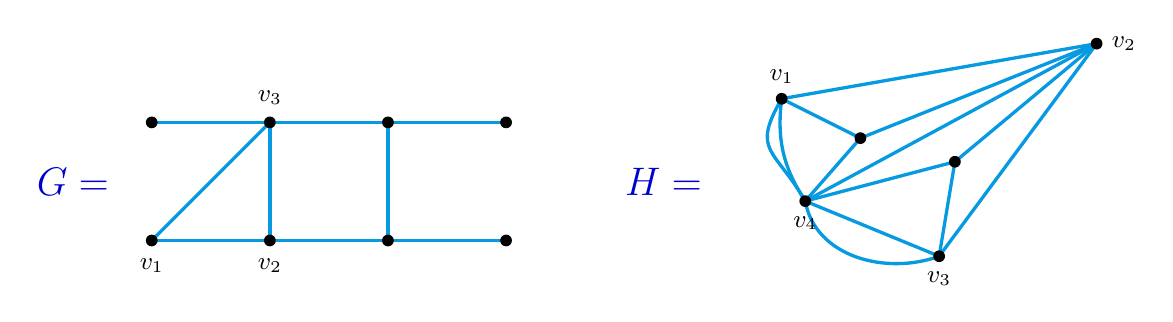
\begin{tikzpicture}[
    % Common Styles
    vertex/.style={
        circle, 
        fill=black, 
        inner sep=1.5pt, 
        outer sep=1pt
    },
    edge/.style={
        cyan!85!blue, 
        line width=1.2pt, 
        line cap=round, 
        line join=round
    },
    label_text/.style={
        font=\sffamily\small, 
        text=black
    },
    title_text/.style={
        font=\Large\sffamily, 
        text=blue!80!black
    }
]

    % ================= GRAPH G =================
    \node[title_text] at (-1, 0.75) {$G=$};

    % Coordinates for grid (2 rows, 4 columns)
    % Bottom Row
    \coordinate (b1) at (0,0);
    \coordinate (b2) at (1.5,0);
    \coordinate (b3) at (3,0);
    \coordinate (b4) at (4.5,0);
    
    % Top Row
    \coordinate (t1) at (0,1.5);
    \coordinate (t2) at (1.5,1.5);
    \coordinate (t3) at (3,1.5);
    \coordinate (t4) at (4.5,1.5);

    % Edges
    % Horizontal rails
    \draw[edge] (t1) -- (t2) -- (t3) -- (t4);
    \draw[edge] (b1) -- (b2) -- (b3) -- (b4);
    
    % Vertical rungs (only at columns 2 and 3 based on sketch)
    \draw[edge] (t2) -- (b2);
    \draw[edge] (t3) -- (b3);
    
    % Diagonal (v1 to v3)
    \draw[edge] (b1) -- (t2);

    % Vertices
    \foreach \p in {b1, b2, b3, b4, t1, t2, t3, t4} {
        \node[vertex] at (\p) {};
    }

    % Labels
    \node[label_text, below=3pt] at (b1) {$v_1$};
    \node[label_text, below=3pt] at (b2) {$v_2$};
    \node[label_text, above=3pt] at (t2) {$v_3$};


    % ================= GRAPH H =================
    \begin{scope}[shift={(8,0)}]
        \node[title_text] at (-1.5, 0.75) {$H=$};

        % Coordinates
        % The Apex (v2 on right)
        \coordinate (hv2) at (4, 2.5);
        
        % The Left Cluster
        \coordinate (hv1) at (0, 1.8);       % Top left
        \coordinate (mid1) at (1, 1.3);      % Internal top
        \coordinate (hv4) at (0.3, 0.5);     % Bottom left
        \coordinate (mid2) at (2.2, 1.0);    % Internal mid
        \coordinate (hv3) at (2, -0.2);      % Bottom right-ish

        % Edges
        % Spanning from Apex (v2)
        \draw[edge] (hv2) -- (hv1);
        \draw[edge] (hv2) -- (mid1);
        \draw[edge] (hv2) -- (mid2);
        \draw[edge] (hv2) -- (hv4);
        \draw[edge] (hv2) -- (hv3);

        % Internal Web
        \draw[edge] (hv1) -- (mid1);
        \draw[edge] (hv1) to[bend right=20] (hv4);
        \draw[edge] (mid1) -- (hv4);
        \draw[edge] (hv4) -- (hv3);
        \draw[edge] (hv4) -- (mid2);
        \draw[edge] (hv3) -- (mid2);

        % The outer curved loop on the left
        \draw[edge] (hv1) to[out=240, in=120, looseness=1.5] (hv4);
        \draw[edge] (hv4) to[out=280, in=200, looseness=1] (hv3);

        % Vertices
        \node[vertex] at (hv2) {};
        \node[vertex] at (hv1) {};
        \node[vertex] at (hv4) {};
        \node[vertex] at (hv3) {};
        \node[vertex] at (mid1) {};
        \node[vertex] at (mid2) {};

        % Labels
        \node[label_text, right=2pt] at (hv2) {$v_2$};
        \node[label_text, above=2pt] at (hv1) {$v_1$};
        \node[label_text, below=2pt] at (hv4) {$v_4$};
        \node[label_text, below=2pt] at (hv3) {$v_3$};

    \end{scope}

\end{tikzpicture}
\end{center}

Then $\omega(G)=3$ witnessed by $\langle \{v_1, v_2, v_3\} \rangle \cong K_3$ and $\omega(H)=4$ witnessed by $\langle \{v_1, v_2, v_3, v_4\} \rangle \cong K_4$, and $H$ being planar.
\end{example}

% 6.26 Lemma
\begin{lemma}
For any graph $G$ we get $\omega(G) \le \chi(G)$.
\end{lemma}
$\to$ Let $\omega(G)=\ell$, then $G$ contains $K_\ell$ as a subgraph which implies that we already need $\ell$ colours just to colour $K_\ell$ and $\ell = \omega(G) \le \chi(G)$.

The question arises whether $\omega(G)$-many colours should always be enough to colour a graph $G$. This hope rather quickly fails, as for example $\omega(C_5)=2$, but $\chi(C_5)=3 > \omega(G)$. Another example is given below.

% 6.27 Example
\begin{example}
Let $G$ be the graph consisting of the disjoint union of $C_5$ and $C_3$ together with all edges between $C_3$ and $C_5$, i.e.
\begin{center}
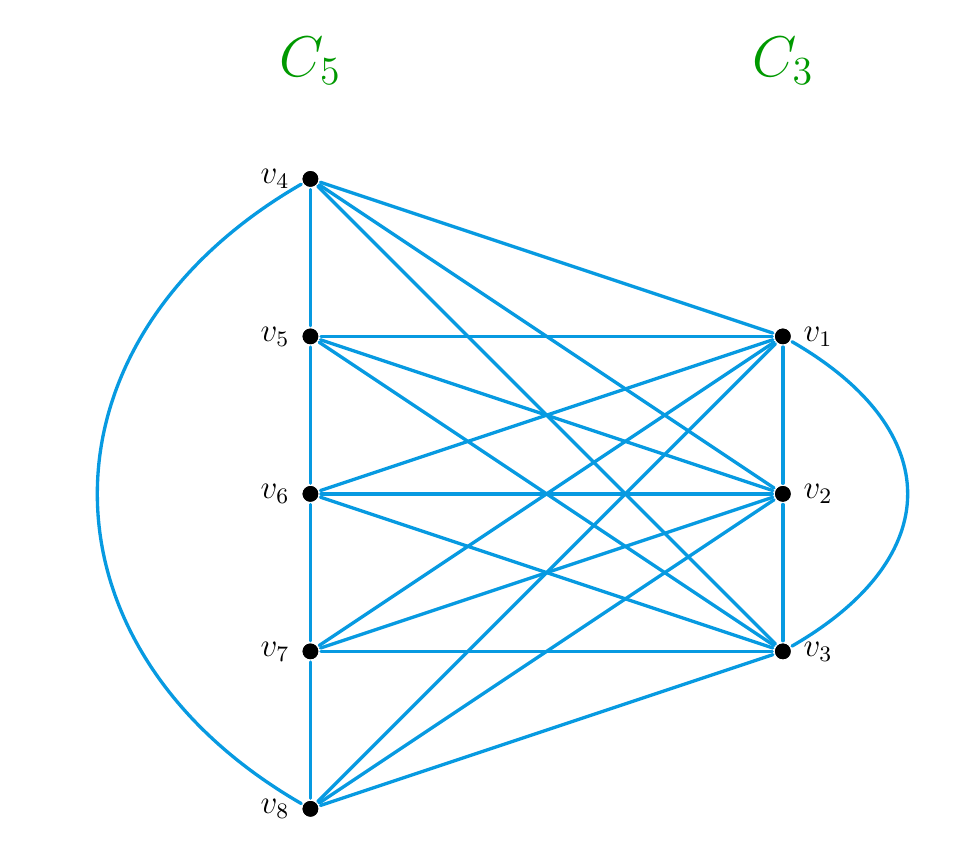
\begin{tikzpicture}[
    % Define styles
    vertex/.style={
        circle, 
        fill=black, 
        inner sep=2pt, 
        outer sep=1pt
    },
    edge/.style={
        cyan!85!blue, 
        line width=1.2pt, 
        line cap=round, 
        line join=round
    },
    label_text/.style={
        font=\sffamily\bfseries\large, 
        text=black
    },
    title_text/.style={
        font=\sffamily\bfseries\huge, 
        text=green!60!black
    }
]

    % --- Left Column (C5) ---
    % Placing vertices v4 to v8
    \node[vertex] (v4) at (0, 4) {};
    \node[vertex] (v5) at (0, 2) {};
    \node[vertex] (v6) at (0, 0) {};
    \node[vertex] (v7) at (0, -2) {};
    \node[vertex] (v8) at (0, -4) {};

    % Labels for C5
    \node[label_text, left=4pt] at (v4) {$v_4$};
    \node[label_text, left=4pt] at (v5) {$v_5$};
    \node[label_text, left=4pt] at (v6) {$v_6$};
    \node[label_text, left=4pt] at (v7) {$v_7$};
    \node[label_text, left=4pt] at (v8) {$v_8$};

    % Title C5
    \node[title_text] at (0, 5.5) {$C_5$};

    % Edges within C5 (Vertical path)
    \draw[edge] (v4) -- (v5) -- (v6) -- (v7) -- (v8);
    % Curved back-edge
    \draw[edge] (v4) to[out=210, in=150, looseness=1.3] (v8);


    % --- Right Column (C3) ---
    % Placing vertices v1 to v3 (Centered vertically relative to left)
    \node[vertex] (v1) at (6, 2) {};
    \node[vertex] (v2) at (6, 0) {};
    \node[vertex] (v3) at (6, -2) {};

    % Labels for C3
    \node[label_text, right=4pt] at (v1) {$v_1$};
    \node[label_text, right=4pt] at (v2) {$v_2$};
    \node[label_text, right=4pt] at (v3) {$v_3$};

    % Title C3
    \node[title_text] at (6, 5.5) {$C_3$};

    % Edges within C3
    \draw[edge] (v1) -- (v2) -- (v3);
    % Curved back-edge
    \draw[edge] (v1) to[out=330, in=30, looseness=1.5] (v3);


    % --- Bipartite Connections ---
    % Connect every node in C5 to every node in C3
    \foreach \leftnode in {v4, v5, v6, v7, v8} {
        \foreach \rightnode in {v1, v2, v3} {
            \draw[edge] (\leftnode) -- (\rightnode);
        }
    }

    % Redraw vertices on top so lines appear behind them
    \foreach \n in {v1,v2,v3,v4,v5,v6,v7,v8} {
        \node[vertex] at (\n) {};
    }

\end{tikzpicture}
\end{center}
Then $\omega(G)=5$, as e.g. $\langle \{v_1, v_2, v_3, v_4, v_5\} \rangle \cong K_5$ (so $\omega(G) \ge 5$), but any 6 vertices need to include at least three vertices from $C_5$, which cannot be mutually incident, so $\omega(G) < 6$, and thus $\omega(G)=5$.
Further, $\chi(G)=6$: The cycle $C_5$ and $C_3$ each need at least 3 colours, and these colours have to be distinct as the vertices are mutually incident.
\end{example}

Let's summarize all bounds we have established.

\topic{Summary}
Let $G$ be any graph of order $n$.
\begin{enumerate}
    \item[1)] $\chi(G) \le \Delta(G) + 1 \le n$.
    \item[2)] If $G$ is connected then $\chi(G) \le \Delta(G)$ iff $G$ is neither complete nor an odd cycle.
    \item[3)] $\omega(G) \le \chi(G)$ and $\frac{n}{\alpha(G)} \le \chi(G) \le n+1-\alpha(G)$.
\end{enumerate}

\section{The 4-Colour Problem}

% 6.28 The Problem
\topic{The Problem (Francis Guthrie, 1852)}
Given any map in the plane - how many colours do we need to colour it in a way s.t. no countries who share part of their border (more than a point) have the same colour?
We can rephrase this in graph theoretic terms. Note that we can represent the issue as a graph where the vertices represent countries and edges connect countries with touching borders. Such a graph will be planar.

% 6.29 Example
\begin{example}
The map
\begin{center}
    \includegraphics[width=0.6\textwidth]{./images/pic_6_29_1.png}
\end{center}
can be represented by the planar graph:

\begin{center}
    \includegraphics[width=0.6\textwidth]{./images/pic_6_29_2.png}
\end{center}

Now, a colouring of the map exactly corresponds to a vertex colouring of the associated graph, e.g.
\begin{center}
    \includegraphics[width=0.6\textwidth]{./images/pic_6_29_3.png}
\end{center}
For this graph, we obtained a 4-colouring. We know that $\omega(G) \le \chi(G)$ for any graph and $\omega(G) \le 4$ for any planar graph. But are 4 colours always enough?
\end{example}

% 6.30 The Four-Colour-Theorem
\begin{theorem}[The Four-Colour-Theorem (1976, Appel, Haken)]
If $G$ is planar, then $\chi(G) \le 4$. I.e. every planar graph is 4-colourable.
\end{theorem}
% 6.31 Some History
\topic{Some History}
\begin{itemize}
    \item 1852 - Problem introduced by Francis Guthrie to De Morgan (his prof).
    \item 1852-1879 Brilliant minds, incl. Hamilton, Cayley, Peirce... tried to solve the problem without success.
    \item 1879 - Alfred Kempe announced a proof.
    \item 1890 - Fatal mistake was found in proof. Soon after - Heawood + Kempe prove that $\chi(G) \le 5$.
    \item 1976 - After 124 years a proof was presented by Appel-Haken. $\to$ relies heavily on computers, not accepted by all mathematicians.
    \item 1996 - Easier proof presented, but still uses computers.
    \item $\to$ The search continues.
\end{itemize}

Maybe somewhat surprisingly, the proof for $\chi(G) \le 5$ is much more accessible. Recall that if $G$ is planar, we have $\delta(G) \le 5$ (Thm 5.17).

% 6.32 Theorem (Renumbered to match your seq if needed, here simply Theorem)
\begin{theorem}
If $G$ is planar, then $\chi(G) \le 5$, i.e. $G$ is 5-colourable.
\end{theorem}

\begin{proof}
Let $|G|=n$. We proceed by induction on $n$.

\vspace{0.3cm}
If $n \le 5$, the theorem clearly holds as $\chi(G) \le |G|$ for any $G$.

\vspace{0.3cm}
\noindent \underline{$n \to n+1$}: Assume any planar graph of order at most $n$ is 5-colourable and consider $G$ s.t. $|G|=n+1$. As $\delta(G) \le 5$, there exists $v \in V_G$ s.t. $\deg(v) \le 5$. Consider the planar graph $G-v$.
By I.H., $G-v$ is 5-colourable. Let $K$ be that 5-colouring. Now, if among the neighbours of $v$ at least one of $\{1, 2, 3, 4, 5\}$ was not used, we can use that colour for $v$ and obtain the desired 5-colouring of $G$.
Otherwise, $\deg(v)=5$ and all neighbours $\{w_1, \dots, w_5\}$ of $v$ are coloured in a different colour, e.g. $K(w_i)=i$. We obtain:
\begin{center}
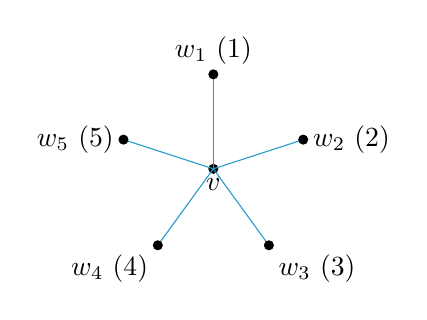
\begin{tikzpicture}[scale=0.8]
    \coordinate (v) at (0,0); \filldraw (v) circle (2pt) node[below] {$v$};
    \foreach \i in {1,...,5} {
        \coordinate (w\i) at (90+72-72*\i : 1.5);
        \draw[cyan!80!black] (v)--(w\i);
        \filldraw (w\i) circle (2pt);
    }
    \node[above] at (w1) {$w_1$ (1)}; \node[right] at (w2) {$w_2$ (2)};
    \node[below right] at (w3) {$w_3$ (3)}; \node[below left] at (w4) {$w_4$ (4)};
    \node[left] at (w5) {$w_5$ (5)};
\end{tikzpicture}
\end{center}
as a subgraph of $G$. Now, we make a case distinction.

\vspace{0.3cm}
\noindent \underline{Case 1}: Assume there is \underline{no} $w_1, w_3$-path that entirely uses vertices coloured with colours 1 and 3. Then let $H$ be the subgraph of $G$ containing all paths that start in $w_1$ and use only vertices of colour 1 and 3, i.e. $H = \bigcup \{P \mid P \text{ is a } w_1 u \text{ path } \& \ K(t) \in \{1, 3\} \forall t \in P\}$.
Note that $w_1 \in H$, but $w_3 \notin H$ by assumption.

\begin{center}
    \includegraphics[width=0.6\textwidth]{./images/pic_6_32_1.png}
\end{center}

Now, in $H$, exchange the colours 1 and 3 and observe that that new colouring $\tilde{K}$ is still a valid colouring for $G$, but now $\tilde{K}(w_1)=3$.
To see that it is valid, assume for contradiction that ex. $x,y$ s.t. $\tilde{K}(x)=\tilde{K}(y)$ and $xy \in E_G$. Then wlog we may assume $x \in H, y \notin H$ and $\tilde{K}(x)=\tilde{K}(y)=1$. But then $K(x)=3, K(y)=1$ and there is a $\{1, 3\}$-coloured $w_1, x$-path $P$. Finally, $P^{\frown}(y)$ would be a $\{1, 3\}$ coloured $w_1, y$-path, whence $y \in H$, contradicting our assumptions.
Hence, $\tilde{K}$ is a 5-colouring of $G-v$, but now the neighbours of $v$ only use colours $\{2, 3, 4, 5\}$, whence we can set $\tilde{K}(v)=1$ and obtain the desired 5-colouring of $G$.

\vspace{0.3cm}
\noindent \underline{Case 2}: Assume there is a $\{1, 3\}$-coloured $w_1 w_3$-path $P$ in $G-v$. As $G$ is planar, we have two options:

\begin{center}
    \includegraphics[width=0.6\textwidth]{./images/pic_6_32_2.png}
\end{center}

In either case, any $w_2 w_4$-path now would have to contain at least one vertex from $P$, as $G$ is planar. But this means that there is no $w_2 w_4$-path which \underline{only} uses colours 2 and 4. We can hence apply Case 1 to $w_2$ and $w_4$ and obtain the desired 5-colouring of $G$.
\end{proof}

\section{Chromatic Polynomials}

% History (Unnumbered)
\par\vspace{0.5cm}\noindent
\needspace{3\baselineskip}
{\large \underline{\textbf{History}}}
\par\vspace{0.2cm}
\begin{itemize}
    \item Introduced 1912 by Georg David Birkhoff to tackle the 4-colour problem (he hoped for a negative answer).
    \item $P_G(k)$ shall describe the number of $k$-colourings of $G$.
    \item These will be polynomials in $k$ of degree $|G|=n$, i.e. $P_G(k) = a_n k^n + \dots + a_1 k + a_0$.
    \item Birkhoff hoped to use strong tools from analysis and algebra to find roots of these polynomials.
    \item In particular, he hoped to find a planar graph $G$ which has $k=4$ as a root, i.e. $P_G(4)=0$, whence $G$ has no 4-colouring, whence the 4-colour theorem would be wrong.
    \item Even though we know that he had no chance of success, he still developed many tools which are crucial in the area of algebraic graph theory.
    \item $\Rightarrow$ Sometimes truly the way is the goal.
\end{itemize}

% 6.33 Definition
\begin{definition}
\begin{enumerate}
    \item[1)] Let $K_1$ and $K_2$ be two colourings of the same graph $G$. We say that $K_1$ is \textbf{\color{red}different} from $K_2$ ($K_1 \ne K_2$) if there is some $v \in V_G$ s.t. $K_1(v) \ne K_2(v)$.
    \item[2)] We denote by \textbf{\color{red}$P_G(k)$} the number of different $k$-colourings of $G$.
\end{enumerate}
\end{definition}

% 6.34 Example
\begin{example}
Consider the following colourings of $K_4$:
\begin{center}
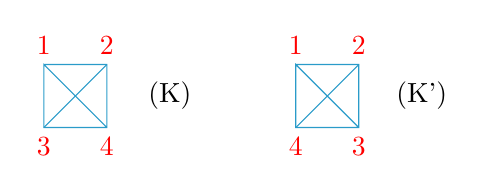
\begin{tikzpicture}[scale=0.8]
    \coordinate (v1) at (0,1); \coordinate (v2) at (1,1);
    \coordinate (v3) at (0,0); \coordinate (v4) at (1,0);
    \draw[cyan!80!black] (v1)--(v2)--(v4)--(v3)--(v1)--(v4); \draw[cyan!80!black] (v2)--(v3);
    \node[red, above] at (v1) {1}; \node[red, above] at (v2) {2};
    \node[red, below] at (v3) {3}; \node[red, below] at (v4) {4};
    
    \node at (2,0.5) {(K)};
    
    \begin{scope}[xshift=4cm]
        \draw[cyan!80!black] (0,1)--(1,1)--(1,0)--(0,0)--(0,1)--(1,0); \draw[cyan!80!black] (1,1)--(0,0);
        \node[red, above] at (0,1) {1}; \node[red, above] at (1,1) {2};
        \node[red, below] at (0,0) {4}; \node[red, below] at (1,0) {3};
        \node at (2,0.5) {(K')};
    \end{scope}
\end{tikzpicture}
\end{center}
Then $K$ and $K'$ are different, as $K(v_3)=3 \ne 4 = K'(v_3)$.
\end{example}

% 6.35 Discussion
\topic{Discussion}
\begin{itemize}
    \item How many 4-colourings of $K_4$ are there?
    $\to$ We can choose any of the 4 colours to colour $v_1$, then any of the remaining 3 for $v_2$ and so on. In the end we obtain $4 \cdot 3 \cdot 2 \cdot 1 = 4!$ many 4-colourings.
    \item What about 6-colourings?
    $\to$ Following the same thoughts, we obtain $6 \cdot 5 \cdot 4 \cdot 3 = \frac{6!}{(6-4)!}$ many 6-colourings.
    \item And 3-colourings?
    $\to$ As $\chi(K_4)=4$, there are no 3-colourings.
\end{itemize}

% 6.36 Definition
\begin{definition}
Let $G$ be any graph. Then we denote by \textbf{\color{red}$P_G(k)$} the number of possible different colourings using at most the colours $\{1, 2, \dots, k\}$.
\end{definition}

% 6.37 Remark
\begin{remark}
\begin{itemize}
    \item Generalising our discussion above, we obtain
    \[ P_{K_n}(k) = \begin{cases} 0 & \text{if } k < n \\ \frac{k!}{(k-n)!} & \text{if } n \le k \end{cases}. \]
    \item Further check quickly that $P_{E_n}(k) = k^n$.
\end{itemize}
\end{remark}

% 6.38 Remark
\begin{remark}
The following are equivalent for any graph $G$ and $k \in \mathbb{Z}_+$:
\begin{enumerate}
    \item[1)] $P_G(k) \ge 1$
    \item[2)] $\chi(G) \le k$
    \item[3)] $G$ is $k$-colourable.
\end{enumerate}
\end{remark}

In order to show that $P_G(k)$ is a polynomial of degree $k$, we need an important observation which will allow us to use inductive arguments. To make sense of it, we need the following definition.

% 6.39 Definition (Edge Contraction)
\begin{definition}[Edge Contraction]
Let $G$ be a graph and $e \in E(G)$, say $e=uv$. Then the \textbf{\color{red}edge contraction $G/e$} is the graph obtained from $G$ by the following:
\begin{enumerate}
    \item[1)] Delete the edge $e$ from $G$, i.e. construct $G-e$.
    \item[2)] Identify the vertices $u$ and $v$ as one new vertex denoted $u \wedge v$.
    \item[3)] Leaving only one copy of any resulting multi-edges.
\end{enumerate}
\end{definition}

% 6.40 Example
\begin{example}
Consider $G$ and $e \in E(G)$ as follows:
\begin{center}
\begin{tikzpicture}[
    % --- Styles ---
    vertex/.style={
        circle, 
        fill=black, 
        inner sep=1.5pt, 
        outer sep=1pt
    },
    edge/.style={
        cyan!85!blue, 
        line width=1.2pt, 
        line cap=round,
        line join=round
    },
    label_text/.style={
        font=\sffamily, 
        text=black
    },
    phrase_text/.style={
        font=\Large\sffamily, 
        text=blue!70!purple,
        align=center
    },
    scale=0.8
]

    % ================= GRAPH 1 (Left) =================
    \begin{scope}[local bounding box=G1]
        % Coordinates
        \coordinate (x4) at (0, -0.2);
        \coordinate (u) at (-0.8, 1.2);
        \coordinate (v) at (0.8, 1.2);
        \coordinate (x1) at (0, 2.2);
        \coordinate (x2) at (-0.8, -1.5);
        \coordinate (x3) at (0.8, -1.5);

        % Edges
        \draw[edge] (u) -- (x1) -- (v);        % Top Triangle sides
        \draw[edge] (u) -- (v) node[midway, above, text=red, font=\small\bfseries] {e}; % Edge e
        \draw[edge] (u) -- (x2) -- (x3) -- (v); % Outer box
        \draw[edge] (x2) -- (x4) -- (x3);       % Bottom internal
        \draw[edge] (u) -- (x4) -- (v);         % Top internal

        % Vertices
        \foreach \n in {x1, x2, x3, x4, u, v} \node[vertex] at (\n) {};

        % Labels
        \node[label_text, above=2pt] at (x1) {$x_1$};
        \node[label_text, left=2pt] at (u) {$u$};
        \node[label_text, right=2pt] at (v) {$v$};
        \node[label_text, below=2pt] at (x2) {$x_2$};
        \node[label_text, below=2pt] at (x3) {$x_3$};
        \node[label_text, right=1pt] at (x4) {$x_4$};
    \end{scope}

    % ================= TEXT 1 =================
    \node[phrase_text, right=0.5cm of G1] (text1) {Then\\$G-e$\\is};

    % ================= GRAPH 2 (Middle: G-e) =================
    \begin{scope}[shift={($(text1.east)+(1.5,0)$)}, local bounding box=G2]
        % Coordinates (same relative positions)
        \coordinate (mx4) at (0, -0.2);
        \coordinate (mu) at (-0.8, 1.2);
        \coordinate (mv) at (0.8, 1.2);
        \coordinate (mx1) at (0, 2.2);
        \coordinate (mx2) at (-0.8, -1.5);
        \coordinate (mx3) at (0.8, -1.5);

        % Edges (Same as G1 but NO u-v edge)
        \draw[edge] (mu) -- (mx1) -- (mv);
        % \draw[edge] (mu) -- (mv);  <-- REMOVED
        \draw[edge] (mu) -- (mx2) -- (mx3) -- (mv);
        \draw[edge] (mx2) -- (mx4) -- (mx3);
        \draw[edge] (mu) -- (mx4) -- (mv);

        % Vertices
        \foreach \n in {mx1, mx2, mx3, mx4, mu, mv} \node[vertex] at (\n) {};

        % Labels
        \node[label_text, above=2pt] at (mx1) {$x_1$};
        \node[label_text, left=2pt] at (mu) {$u$};
        \node[label_text, right=2pt] at (mv) {$v$};
        \node[label_text, below=2pt] at (mx2) {$x_2$};
        \node[label_text, below=2pt] at (mx3) {$x_3$};
        \node[label_text, below=1pt] at (mx4) {$x_4$};
    \end{scope}

    % ================= TEXT 2 =================
    \node[phrase_text, right=0.5cm of G2] (text2) {and\\$G/e$\\is};

    % ================= GRAPH 3 (Right: G/e) =================
    \begin{scope}[shift={($(text2.east)+(1.5,0)$)}]
        % Coordinates
        \coordinate (rx4) at (0, -0.5);
        \coordinate (ruv) at (0, 1.2); % Merged u and v
        \coordinate (rx1) at (0, 2.2);
        \coordinate (rx2) at (-1.0, -1.5); % Slightly wider to match triangle shape
        \coordinate (rx3) at (1.0, -1.5);

        % Edges
        \draw[edge] (rx1) -- (ruv);              % Top stem
        \draw[edge] (ruv) -- (rx4);              % Center stem
        \draw[edge] (rx2) -- (rx3);              % Bottom base
        \draw[edge] (rx2) -- (rx4) -- (rx3);     % Internal V

        % Outer connections (curved slightly to look natural)
        \draw[edge] (ruv) -- (rx2);
        \draw[edge] (ruv) -- (rx3);

        % Vertices
        \foreach \n in {rx1, rx2, rx3, rx4, ruv} \node[vertex] at (\n) {};

        % Labels
        \node[label_text, right=2pt] at (rx1) {$x_1$};
        \node[label_text, right=2pt] at (ruv) {$u \cdot v$};
        \node[label_text, below=2pt] at (rx2) {$x_2$};
        \node[label_text, below=2pt] at (rx3) {$x_3$};
        \node[label_text, right=2pt] at (rx4) {$x_4$};
    \end{scope}

\end{tikzpicture}
\end{center}
\end{example}

% 6.41 Theorem
\begin{theorem}[Birkhoff, Lewis, 1946]
Let $G$ be any non-empty graph and $e=uv \in E(G)$. Then
\[ P_G(k) = P_{G-e}(k) - P_{G/e}(k). \]
\end{theorem}

\begin{proof}
\underline{Claim 1}: $P_{G/e}(k)$ is equal to the number of $k$-colourings of $G-e$ which assign the same colour to $u$ and $v$.
$\to$ Let $K$ be a $k$-colouring of $P_{G/e}$. Then we can create a $k$-colouring $\tilde{K}$ of $G-e$ via
\[ \tilde{K}(x) = \begin{cases} K(u \wedge v) & \text{if } x=u \text{ or } x=v \\ K(x) & \text{otherwise}. \end{cases} \]
Hence, there are at least as many $k$-colourings of $G-e$ which assign the same colour to $u$ and $v$ as there are $k$-colourings of $G/e$.
On the other hand, if $\tilde{K}$ is any $k$-colouring of $G-e$ which assigns the same colour to $u$ and $v$, then we can define a new $k$-colouring $K$ of $G/e$ by setting
\[ K(x) = \begin{cases} \tilde{K}(u) & \text{if } x=u \wedge v \\ \tilde{K}(x) & \text{else}. \end{cases} \]
Hence, there are at least as many $k$-colourings of $G/e$ as there are $k$-colourings of $G-e$ assigning the same colour to $u$ and $v$.

\underline{Claim 2}: There are as many $k$-colourings of $G$ as there are $k$-colourings of $G-e$ assigning different colours to $u$ and $v$.
$\to$ If $\tilde{K}$ is a $k$-colouring of $G$, then clearly it is a $k$-colouring of $G-e$ assigning different colours to $u$ and $v$. And vice versa.

Now,
\begin{align*}
    P_{G-e}(k) &= |\{K \mid K \text{ is a } k\text{-colouring of } G-e\}| \\
    &= |\{K \mid K \text{ $k$-colouring of } G-e \text{ with } K(u)=K(v)\}| \\
    &+ |\{K \mid K \text{ $k$-colouring of } G-e \text{ with } K(u) \ne K(v)\}| \\
    &= P_{G/e}(k) + P_G(k).
\end{align*}
Thus, $P_G(k) = P_{G-e}(k) - P_{G/e}(k)$, as desired.
\end{proof}

% 6.42 Remark
\begin{remark}
Combinatorics seems faster than Birkhoff-Lewis, so why bother?
\begin{enumerate}
    \item[1)] We do not need to always reduce back to $E_n$, once we know the chromatic polynomial of other graphs $\to$ it becomes much faster.
    \item[2)] It allows inductive arguments in proofs (see below).
    \item[3)] Combinatorial thoughts depend on the choice of vertices and hence do not always give the correct number!
    \\[0.2cm]
    e.g. $G=$
    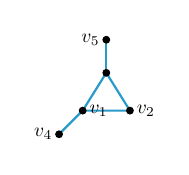
\begin{tikzpicture}[baseline=-0.5ex, scale=0.6]
        \coordinate (v1) at (0,0); 
        \coordinate (v2) at (1,0); 
        \coordinate (top) at (0.5, 0.8);
        \coordinate (v4) at (-0.5, -0.5); 
        \coordinate (v5) at (0.5, 1.5);
        
        \draw[cyan!80!black, thick] (v1)--(v2)--(top)--(v1);
        \draw[cyan!80!black, thick] (v1)--(v4);
        \draw[cyan!80!black, thick] (top)--(v5); % v2v5 in note text, but drawing connects top node
        
        \foreach \p in {v1,v2,top,v4,v5} \filldraw (\p) circle (2pt);
        \node[right, scale=0.7] at (v1) {$v_1$}; 
        \node[right, scale=0.7] at (v2) {$v_2$};
        \node[left, scale=0.7] at (v4) {$v_4$};
        \node[left, scale=0.7] at (v5) {$v_5$};
    \end{tikzpicture}
    $P_G(3) \dots$ there are 3 colours to pick from for $v_5$, also 3 for $v_4$, 2 for $v_1$, 2 for $v_3$ and either 1 or 0 for $v_2 \dots$ we need a case distinction! \\
    $\leadsto$ Things get messy very quickly.
\end{enumerate}

\vspace{0.3cm}
\noindent \underline{But:} Applying Birkhoff-Lewis, we always get a solid solution!

Note: $P_{C_3}(3) = 3^3 - 3 \cdot 3^2 + 2 \cdot 3 = 6$. Now set $e_1 := v_1 v_4$, $e_2 := v_2 v_5$.

% Visual Grid for G0...G11
\begin{center}
\begin{tabular}{l l}
    Then $G_0 := G-e_1$ is
    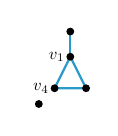
\begin{tikzpicture}[baseline=-0.5ex, scale=0.4]
        \coordinate (a) at (0,0); \coordinate (b) at (1,0); \coordinate (c) at (0.5,1); \coordinate (d) at (0.5,1.8); \coordinate (v4) at (-0.5, -0.5);
        \draw[cyan!80!black, thick] (a)--(b)--(c)--(a); \draw[cyan!80!black, thick] (c)--(d);
        \foreach \p in {a,b,c,d,v4} \filldraw (\p) circle (3pt);
        \node[left, scale=0.6] at (a) {$v_4$}; \node[left, scale=0.6] at (c) {$v_1$};
    \end{tikzpicture}
    , & 
    $G_1 := G/e_1$ is
    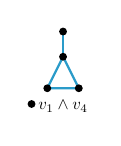
\begin{tikzpicture}[baseline=-0.5ex, scale=0.4]
        \coordinate (a) at (0,0); \coordinate (b) at (1,0); \coordinate (c) at (0.5,1); \coordinate (d) at (0.5,1.8);
        \coordinate (v4) at (-0.5, -0.5);
        \draw[cyan!80!black, thick] (a)--(b)--(c)--(a); \draw[cyan!80!black, thick] (c)--(d);
        \foreach \p in {a,b,c,d,v4} \filldraw (\p) circle (3pt);
        \node[below, scale=0.6] at (0.5, -0.2) {$v_1 \wedge v_4$};
    \end{tikzpicture}
    \\[0.8cm]
    
    Further $G_{00} := G_0-e_2$ is
    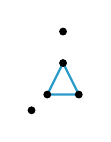
\begin{tikzpicture}[baseline=-0.5ex, scale=0.4]
        \coordinate (a) at (0,0); \coordinate (b) at (1,0); \coordinate (c) at (0.5,1);
        \coordinate (v4) at (-0.5, -0.5);
        \draw[cyan!80!black, thick] (a)--(b)--(c)--(a); % Triangle
        \filldraw (0.5, 2) circle (3pt); % Isolated v5
        \foreach \p in {a,b,c,v4} \filldraw (\p) circle (3pt);
    \end{tikzpicture}
    , &
    $G_{01} := G_0/e_2$ is
    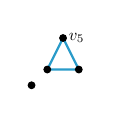
\begin{tikzpicture}[baseline=-0.5ex, scale=0.4]
        \coordinate (a) at (0,0); \coordinate (b) at (1,0); \coordinate (c) at (0.5,1);
        \coordinate (v4) at (-0.5, -0.5);
        \draw[cyan!80!black, thick] (a)--(b)--(c)--(a); % Triangle
        \node[right, scale=0.6] at (c) {$v_5$};
        \foreach \p in {a,b,c,v4} \filldraw (\p) circle (3pt);
    \end{tikzpicture}
    \\[0.8cm]
    
    and $G_{10} := G_1-e_2$ is
    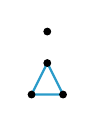
\begin{tikzpicture}[baseline=-0.5ex, scale=0.4]
        \coordinate (a) at (0,0); \coordinate (b) at (1,0); \coordinate (c) at (0.5,1);
        \draw[cyan!80!black, thick] (a)--(b)--(c)--(a);
        \filldraw (0.5, 2) circle (3pt); % Isolated
        \foreach \p in {a,b,c} \filldraw (\p) circle (3pt);
    \end{tikzpicture}
    , & 
    $G_{11} := G_1/e_2$ is
    
\begin{tikzpicture}[baseline=-0.5ex, scale=0.4]
        \coordinate (a) at (0,0); \coordinate (b) at (1,0); \coordinate (c) at (0.5,1);
        \draw[cyan!80!black, thick] (a)--(b)--(c)--(a);
        \foreach \p in {a,b,c} \filldraw (\p) circle (3pt);
    \end{tikzpicture}
\end{tabular}
\end{center}

\begin{align*}
    \text{Now } P_G(3) &= P_{G_0}(3) - P_{G_1}(3) = P_{G_{00}}(3) - P_{G_{01}}(3) - (P_{G_{10}}(3) + P_{G_{11}}(3)) \\
    &= 3 \cdot 3 \cdot 6 - 3 \cdot 6 - 3 \cdot 6 + 6 \\
    &= 6(9 - 3 - 3 + 1) = 24.
\end{align*}
\end{remark}

% 6.43 Theorem
\begin{theorem}
Let $G$ be a graph of order $n$. The following hold.
\begin{enumerate}
    \item[1)] $P_G(k)$ is a polynomial in $k$ of degree $n$, $P_G(k) = a_n k^n + \dots + a_1 k + a_0$.
    \item[2)] We always have $a_n=1$ and $a_0=0$, i.e. $P_G(k) = k^n + a_{n-1}k^{n-1} + \dots + a_1 k$.
    \item[3)] The $a_i$ alternate in sign and $a_{n-1} = -|E(G)|$.
\end{enumerate}
\end{theorem}